\documentclass{article}
\usepackage{tikz, comment}
\usepackage{pifont}
\usepackage{fontspec}
\usetikzlibrary{arrows, decorations.markings, decorations.pathreplacing}
\begin{comment}
:Title: Not defined yet
:Tags: approximation by differentials;equation of a line;inverse variation, inverse proportion , inversely proportional ;average rate of change, arc ;area using parametric equations,parametric integral formula
:Prob: 0.5163;0.4954;0.4536;0.441;0.4401
:Slug: No name yet

Description Here.........
\end{comment}
\begin{document}\centering

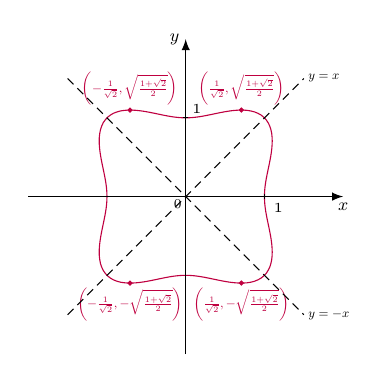
\begin{tikzpicture}[>=latex,xscale=.5*2, yscale=.5*2][font=\sf\small]

%\draw[xstep=1cm,ystep=1cm,color=gray!80] (0, -1) grid (8, 8);

%\clip[] (-3, -4.5) rectangle (6, 4.5);
\draw[purple, samples=100, smooth, domain=0:2*pi, variable=\t]
plot ({sqrt(1/((cos(\t r))^4+(sin(\t r))^4))*cos(\t r)}, {sqrt(1/((cos(\t r))^4+(sin(\t r))^4))*sin(\t r)});

\draw[purple, fill, xscale=1/2, yscale=1/2] ({1/sqrt(2)*2}, {sqrt((1+sqrt(2))/2)*2}) circle(0.05)node[above, scale=0.5]{$\left(\frac{1}{\sqrt 2}, \sqrt{\frac{1+\sqrt{2}}{2}} \right)$};

\draw[purple, fill, xscale=1/2, yscale=1/2] ({-1/sqrt(2)*2}, {sqrt((1+sqrt(2))/2)*2}) circle(0.05)node[above, scale=0.5]{$\left(-\frac{1}{\sqrt 2}, \sqrt{\frac{1+\sqrt{2}}{2}} \right)$};

\draw[purple, fill, xscale=1/2, yscale=1/2] ({1/sqrt(2)*2}, {-sqrt((1+sqrt(2))/2)*2}) circle(0.05)node[below, scale=0.5]{$\left(\frac{1}{\sqrt 2}, -\sqrt{\frac{1+\sqrt{2}}{2}} \right)$};

\draw[purple, fill, xscale=1/2, yscale=1/2] ({-1/sqrt(2)*2}, {-sqrt((1+sqrt(2))/2)*2}) circle(0.05)node[below, scale=0.5]{$\left(-\frac{1}{\sqrt 2}, -\sqrt{\frac{1+\sqrt{2}}{2}} \right)$};

\draw[densely dashed] (-1.5, -1.5)--(1.5, 1.5)node[right, scale=0.5]{$y=x$};
\draw[densely dashed] (-1.5, 1.5)--(1.5, -1.5)node[right, scale=0.5]{$y=-x$};

\foreach \x in {}
\draw (\x,2pt/2) -- (\x,-2pt/2)
node[anchor=north] {}%{\tiny$\x$}
;
\draw (1,2pt/2) -- (1,-2pt/2) node[right, yshift=-3] {\tiny$1$};

\foreach \x in {}
\draw (\x,2pt/2) -- (\x,-2pt/2)
node[anchor=south] {\tiny$\x$}
;
\foreach \y in {}
\draw (-2pt/2,\y) -- (2pt/2,\y)
node[anchor=east] {}%{\tiny $\y$}
;
\draw (2pt/2, 1) -- (-2pt/2,1) node[right, yshift=3] {\tiny$1$};

\draw[->] (-2, 0) -- (2, 0)node[below, scale=0.7] {$x$};
\draw[->] (0, -2) -- (0, 2)node[left, scale=0.7] {$y$};

\node[scale=0.7] at ({-0.2/2}, {-0.2/2}) {\scriptsize$0$};

\end{tikzpicture}
\end{document}